\textbf{See the instruction for questions \inteval{\value{question}+1} to \inteval{\value{question}+2}.}

\begin{figure}[H]
\centering
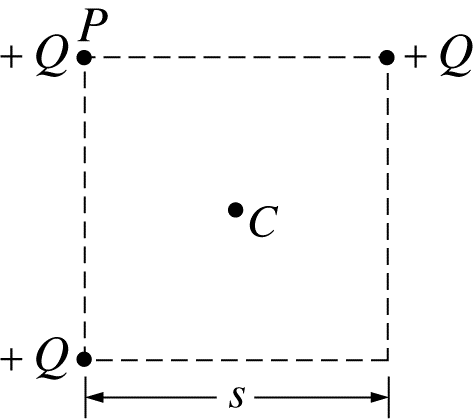
\includegraphics[scale=0.25]{images/img-002-002.png}
\end{figure}

Three particles each with charge $+Q$ are placed on three corners of a square, as shown above. The sides of the square have length $s$. Point $C$ is at the center of the square.

% Multiple Choice Question 2
\begin{questions}\setcounter{question}{1}\question
What is the direction of the electric field at point $C$ ?

\begin{oneparchoices}
\choice \adjustbox{valign=t}{
\includegraphics[scale=0.3]{images/img-002-003.png}}
\choice \adjustbox{valign=t}{
\includegraphics[scale=0.3]{images/img-002-004.png}}
\choice \adjustbox{valign=t}{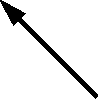
\includegraphics[scale=0.3]{images/img-002-005.png}}
\choice \adjustbox{valign=t}{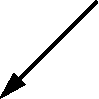
\includegraphics[scale=0.3]{images/img-002-006.png}}
\choice \adjustbox{valign=t}{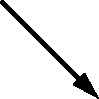
\includegraphics[scale=0.3]{images/img-002-007.png}}
\end{oneparchoices}\end{questions}

% Multiple Choice Question 3
\begin{questions}\setcounter{question}{2}\question
The particle at corner $P$ is allowed to move while the other two particles are held in place. What is the work done by the electric field as the particle at corner $P$ moves to infinity?

\begin{oneparchoices}
\choice $\dfrac{2 k Q^{2}}{s}$
\choice $\dfrac{2 k Q}{s}$
\choice $\dfrac{k Q}{s^{2}}$
\choice $\dfrac{k Q^{2}}{s^{2}}$
\choice $\dfrac{2 k Q^{2}}{s^{2}}$
\end{oneparchoices}\end{questions}

